\chapter{Tests}

\paragraph{}
L'ensemble des tests ont été réalisés via l'utilisation de machines virtuelles,
mais ils auraient pu être reproduits sur de vraies machines.

\section{Mise en place}

\paragraph{}
Dans le but de correctement tester la compatibilité entre les deux systèmes, il
est nécessaire d'installer chacun d'eux, de telle sorte qu'ils aient un disque
en commun.

\subsection{Installation des systèmes}
\subsubsection{Linux}
Le système Linux utilisé peut être n'importe-quelle distribution, tant qu'il est
possible d'y gérer des disques chiffrés avec le standard \textit{LUKS 1}. Pour
cela, il est nécessaire que \texttt{cryptsetup} soit installé. La machine ne
servira ensuite plus qu'à créer les volumes chiffrés avec différents algorithmes
afin de tester leur déchiffrement depuis FreeBSD.
\subsubsection{FreeBSD}
Nous nous sommes basé sur la dernière version stable de FreeBSD à ce jour, à
savoir la version \textit{11.2-RELEASE}. Il est directement possible d'y
compiler un nouveau noyau ainsi que ses utilitaires à partir du code source.

\subsection{Création des partions chiffrées}
\paragraph{}
Les partitions chiffrées sont créées depuis le système Linux sur un disque
séparé et enregistré en tant qu'image disque virtuelle. Les partitions créées
sont:
\begin{itemize}
\item une partition chiffrée \texttt{aes-xts-plain64}
\item une partition chiffrée \texttt{aes-cbc-plain}
\item une partition chiffrée \texttt{aes-cbc-essiv:sha256}
\item une partition chiffrée \texttt{cast5-cbc-plain}
\item une partition en clair
\end{itemize}
\paragraph{}
Après avoir créé différentes partitions à l'aide d'un outils comme
\texttt{cfdisk}, il est possible d'y créer un système chiffré LUKS. Les
commandes utilisées afin de créer les différentes partitions chiffrées sous
Linux sont:
\\
\begin{lstlisting}[language=bash]
  # Linux
  
  cryptsetup luksFormat -c aes-xts-plain64 /dev/sdb1
  cryptsetup luksFormat -c aes-cbc-plain /dev/sdb2
  cryptsetup luksFormat -c aes-cbc-essiv:sha256 /dev/sdb3
  cryptsetup luksFormat -c cast5-cbc-plain /dev/sdb4
\end{lstlisting}
\paragraph{}
Il est ensuite possible de déchiffrer les partitions pour les formater et y
écrire des données. Cela permettra de vérifier par la suite que notre
implémentation de \textit{LUKS} sur FreeBSD est bien capable de le lire.
\\
\begin{lstlisting}[language=bash]
  # Linux
  
  cryptsetup luksOpen /dev/sdb1 luks_device
  mkfs.ext2 /dev/sdb1 # necessaire qu'au moment de la creation du volume
  mount /dev/mapper/luks_device /mnt
  echo "geom_luks: aes-xts-plain64 OK" > /mnt/file.txt
  umount /mnt
  cryptsetup luksClose luks_device
\end{lstlisting}
\paragraph{}
Une fois les partitions chiffrées créées sur un disque, on peut l'ajouter à la
machine fonctionnant sous FreeBSD, qui pourra ainsi directement interagir
directement avec lui.
\paragraph{}
Pour plus de simplicité mais des tests équivalents, il est également possible
d'utiliser des fichiers et d'y héberger les systèmes chiffrés. Cette opération
est réalisable sous Linux cette manière:
\\
\begin{lstlisting}[language=bash]
  # Linux
  
  # creation du fichier
  dd if=/dev/zero of=file bs=1M count=10
  losetup -a /dev/loop0 file
  cryptsetup luksFormat -c aes-xts-plain64 /dev/loop0
  cryptsetup luksOpen /dev/loop0 luks_device
  mkfs.ext2 /dev/mapper/luks_device

  # effectuer les actions voulues sur /dev/loop0
  # (dechiffrement, montage, lecture, ecriture, ...)

  cryptsetup luksClose luks_device
  losetup -d /dev/loop0
\end{lstlisting}
\paragraph{}
Une fois les partitions créées et formatées, seule la commande
\texttt{cryptsetup luksOpen} est nécessaire avant de monter le volume. Chacune
de ces partitions contient un système de fichiers \texttt{ext2}, lisible
directement sur FreeBSD grâce au module noyau \textit{Ext2fs} via la commande
\texttt{mount -t ext2fs /dev/ada1p1 /mnt} (\texttt{/dev/ada1p1} étant
l'emplacement du volume à monter dans \texttt{/mnt/}; figure
\ref{fig:linux_partitions}).
\begin{figure}[H]
  \centering
  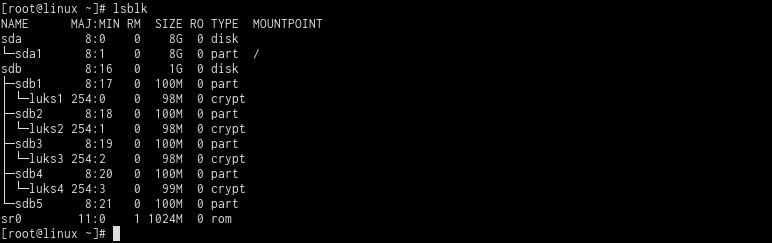
\includegraphics[width=\linewidth]{tests/linux_partitions.png}
  \caption{\label{fig:linux_partitions}Création des partitions}
\end{figure}
Dans le cas où on utilise d'un fichier qu'on aurait copié dans le répertoire
courant, il faut d'abord l'attacher en tant que disque avec l'outil
\texttt{mdconfig}.
\\
\begin{lstlisting}[language=bash]
  # FreeBSD
  
  # attacher le fichier
  mdconfig -a file -u 0

  # detacher le fichier
  mdconfig -d -u 0
\end{lstlisting}
\paragraph{}
\texttt{-u 0} permet d'indiquer que l'emplacement \texttt{/dev/md0} sera
utilisé.

\section{Tests des différentes fonctionnalités}

\subsection{Lecture des métadonnées}
\paragraph{}
Dans un premier temps, afin de tester la lecture de métadonnées sans devoir se
préocuper des difficultés posées par la lecture de disque (notamment dues à
l'emplacement des métadonnées qui diffère entre \textit{LUKS} et \textit{GELI}),
nous avons créé des fichiers contenant un volume chiffré. Pour ce faire, on
copie dans un fichier les données d'une des partitions chiffrées \textit{LUKS}
créées précédemment. Cette opération est directement réalisée sur FreeBSD. On
tente ensuite d'afficher les métadonnées présentes sur ce fichier.
\\
\begin{lstlisting}[language=bash]
  # Linux

  cryptsetup luksDump /dev/sdb1
\end{lstlisting}
\begin{lstlisting}[language=bash]
  # FreeBSD
  
  dd if=/dev/ada1p1 of=file bs=1M
  gluks dump_raw file
\end{lstlisting}
\paragraph{}
Cela permet de vérifier que la structure utilisée est cohérente et que les types
de ses variables sont corrects. Pour cela, on utilise les commandes réalisant
cette opérations et on compare leur sortie sur les deux systèmes (figures
\ref{fig:linux_dump_file} et \ref{fig:freebsd_dump_file}).
\begin{figure}[H]
  \centering
  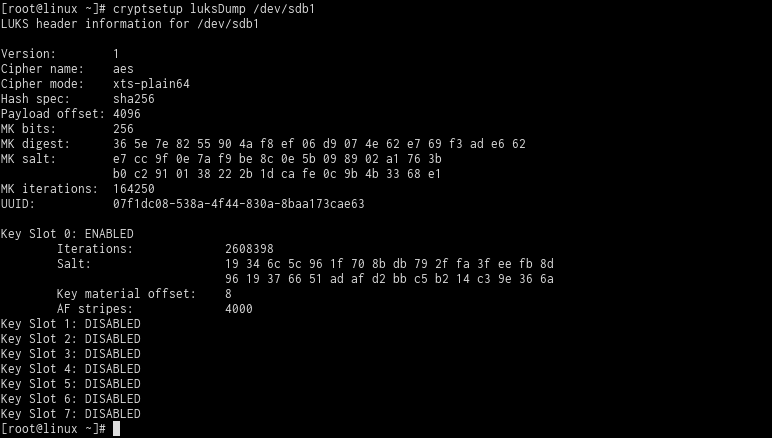
\includegraphics[width=\linewidth]{tests/linux_dump_disk.png}
  \caption{\label{fig:linux_dump_file}Affichage des métadonnées sur Linux}
\end{figure}
\begin{figure}[H]
  \centering
  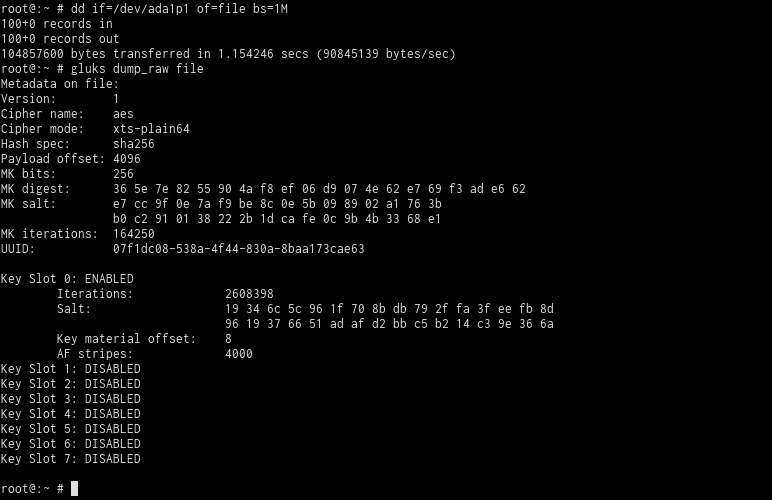
\includegraphics[width=\linewidth]{tests/freebsd_dump_file.png}
  \caption{\label{fig:freebsd_dump_file}Affichage des métadonnées sur FreeBSD
    depuis un fichier}
\end{figure}

\paragraph{}
Une fois que la structure des métadonnées utilisée a été vérifiée et validée, on
peut poursuivre les tests sur une \textit{vraie} partition chiffrée. Pour ce
faire, on peut utiliser les partitions chiffrées \textit{LUKS} qui sont
accessibles depuis notre système FreeBSD (figure \ref{fig:freebsd_dump_disk}).
\\
\begin{lstlisting}[language=bash]
  # FreeBSD

  gluks dump_raw /dev/ada1p1
\end{lstlisting}
\begin{figure}[H]
  \centering
  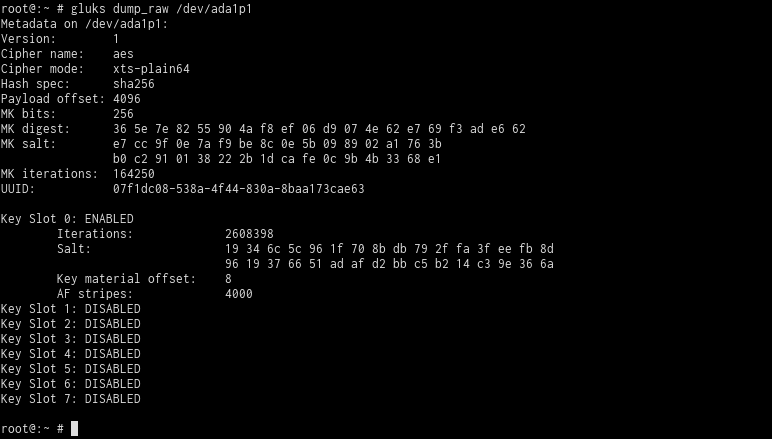
\includegraphics[width=\linewidth]{tests/freebsd_dump_disk.png}
  \caption{\label{fig:freebsd_dump_disk}Affichage des métadonnées sur FreeBSD
    depuis un disque}
\end{figure}

\subsection{Déchiffrement de la clé maître}
\paragraph{}
Pour tester le déchiffrement de la clé maître (ou \textit{masterkey}), on part
de la fonction \texttt{geli attach}, responsable du déchiffrement et de
l'attachement d'un volume chiffré, en enlevant dans un premier temps la partie
de la fonction s'occupant de l'attachement.
\paragraph{}
Sous FreeBSD, l'attachement de volume avec \textit{GELI} consiste en son
déchiffrement et le fait de le rendre disponible au montage. Une fois déchiffré,
un fichier ayant pour extension \texttt{.eli} (ou \texttt{.luks} dans notre
outil) est créé: c'est lui qui pourra ensuite être monté comme n'importe-quel
autre volume non chiffré. Sur un système Linux, ce fichier correspond à celui
créé dans \texttt{/dev/mapper/} grâce à \texttt{cryptsetup luksOpen}. Cette
opération est donc ignorée pour l'instant.
\paragraph{}
Les fonctions réalisant le déchiffrement de la clé maître à partir d'une phrase
secrète permettent de savoir si celle-ci est correcte où non. Il est donc
possible de savoir si le déchiffrement se fait correctement, sans même avoir
besoin de monter le disque pour vérifier son contenu (figure
\ref{fig:freebsd_test_passphrase}).
\\
\begin{lstlisting}[language=bash]
  # FreeBSD

  gluks test_passphrase /dev/ada1p1
\end{lstlisting}
\begin{figure}[H]
  \centering
  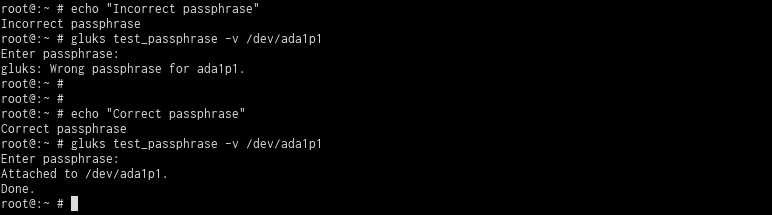
\includegraphics[width=\linewidth]{tests/freebsd_test_passphrase.png}
  \caption{\label{fig:freebsd_test_passphrase}Test de déchiffrement de la clé maître}
\end{figure}
\paragraph{}
Dans le premier cas, une phrase secrète incorrecte a été entrée. Le système
n'arrivant pas à déchiffrer la clé maître à partir de cette phrase, il a donc
pas attaché le volume.
\paragraph{}
Dans le second cas, la phrase entrée était correcte. Le système a donc pu
déchiffrer la clé maître et a attaché le volume, en créant un fichier
d'extension \texttt{.luks}.

\subsection{Montage et lecture de données}
\paragraph{}
Maintenant qu'il est possible de déchiffrer la clé maître, responsable du
chiffrement du disque, à partir d'une des phrases secrètes, il faut s'assurer du
bon déchiffrement du disque en tant que tel.
\paragraph{}
On reprend la fonction précédente pour y ajouter cette fois-ci la partie
responsable de l'attachement du volume chiffré. Après s'être assuré qu'un
fichier en \texttt{.luks} est bien créé dans \texttt{/dev/}, son montage dans
l'arborescence peut se faire. Cette action est réalisée via la commande
\texttt{mount -t ext2fs /dev/ada1p1.luks /mnt}. On peut ensuite s'assurer de son
contenu, en vérifiant par exemple celui d'un fichier texte qu'on aurait créé
sous Linux.

\subsection{Montage et écriture de données}
\paragraph{}
De même, une fois le volume déchiffré monté, il doit être possible d'y écrire
des données. On peut par exemple y placer un fichier contenant du texte.
\paragraph{}
Il est ensuite possible de vérifier son contenu depuis notre machine Linux, en
ouvrant le disque avec \texttt{cryptsetup} puis en le montant.